% -*- coding: utf-8 -*-
%%%%%%%%%%%%%%%%%%%%%%%%%%%%%%%%%%%%%%%%%%%%%%%%%%%%%%%%%%%%%%%%%%%%%%%%%%%%%%%%
%2345678901234567890123456789012345678901234567890123456789012345678901234567890
%        1         2         3         4         5         6         7         8

%\UseRawInputEncoding


%\documentclass[letterpaper, 10 pt, conference]{ieeeconf}  % Comment this line out if you need a4paper
\documentclass[letterpaper, 10 pt, conference]{ieeeconf}
%\pdfminorversion=4              % tell pdflatex to generate PDF in version 1.4
\usepackage[T1]{fontenc}
\usepackage{cite}
\usepackage{amssymb,amsfonts}
\usepackage{algorithmic}
\usepackage{graphicx}
\usepackage{textcomp}
\usepackage{changes}
\usepackage{subcaption}
\usepackage{xcolor}
\usepackage{color, soul}
\usepackage{amsmath}
\usepackage{booktabs}
\usepackage{multirow}
\usepackage{xstring}
%\documentclass[a4paper, 10pt, conference]{ieeeconf}      % Use this line for a4 paper

\IEEEoverridecommandlockouts                              % This command is only needed if 
                                                          % you want to use the \thanks command

\overrideIEEEmargins                                      % Needed to meet printer requirements.

%In case you encounter the following error:
%Error 1010 The PDF file may be corrupt (unable to open PDF file) OR
%Error 1000 An error occurred while parsing a contents stream. Unable to analyze the PDF file.
%This is a known problem with pdfLaTeX conversion filter. The file cannot be opened with acrobat reader
%Please use one of the alternatives below to circumvent this error by uncommenting one or the other
%\pdfobjcompresslevel=0
%\pdfminorversion=4

% See the \addtolength command later in the file to balance the column lengths
% on the last page of the document

% The following packages can be found on http:\\www.ctan.org
%\usepackage{graphics} % for pdf, bitmapped graphics files
%\usepackage{epsfig} % for postscript graphics files
%\usepackage{mathptmx} % assumes new font selection scheme installed
%\usepackage{times} % assumes new font selection scheme installed
%\usepackage{amsmath} % assumes amsmath package installed
%\usepackage{amssymb}  % assumes amsmath package installed
\usepackage{cite}
\usepackage{caption}
\title{\LARGE \bf
RONet: Real-time Range-only Indoor Localization via Stacked Bidirectional LSTM with Residual Attention}

\author{Hyungtae Lim$^{1}$ , Changgue Park$^{2}$, Hyun Myung$^{3}$, \textit{Senior Member, IEEE}% <-this % stops a space
\thanks{
	*This study was supported by the Ministry of Trade, Industry \& Energy(MOTIE, Korea) based on the Industrial Technology Innovation Program. No.10067202, 'Development of Disaster Response Robot System for Lifesaving and Supporting Fire Fighters at Complex Disaster Environment'.}% <-this % stops a space
\thanks{$^{1}$Hyungtae Lim, $^{2}$Changgue Park, and $^{3}$Hyun Myung are with
	the Urban Robotics Laboratory, Korea Advanced Institute of Science
	and Technology (KAIST) Daejeon, 34141, South Korea. {\tt\small shapelim@kaist.ac.kr, cpark@kaist.ac.kr, hmyung@kaist.ac.kr}}%
%
}

\begin{document}

\captionsetup[figure]{labelformat={default},labelsep=period,name={fig.}}

\maketitle
\thispagestyle{empty}
\pagestyle{empty}

%%%%%%%%%%%%%%%%%%%%%%%%%%%%%%%%%%%%%%%%%%%%%%%%%%%%%%%%%%%%%%%%%%%%%%%%%%%%%%%%
\begin{abstract}

In this study, a three-layered bidirectional Long Short-term Memory (Bi--LSTM) with residual attention, named as RONet, is proposed to achieve localization using range measurements. Accordingly, we acquired our own datasets and tested RONet using realistic conditions. It is shown that the RONet can estimate the position of the mobile robot in real time using the Nvidia Jetson AGX Xavier based only on range measurements. We also analyzed the sequence length of LSTM as a type of hyperparameters. We found that a sequence with a length equal to eight is optimal compared to sequences with different lengths, given that construction of the network with the optimal sequence length estimates the position precisely and accounts for uncertainties. As verified experimentally, RONet yields more precise performance and results in increased robustness against outliers compared to a conventional range-only approach based on a particle filtering and the other conventional deep-learning-based approaches. We set three cases, reduced the number of anchors, and verified that the RONet was a robust solution. We also confirmed that it is the best solution that yields the smallest Root-Mean-Square-Error (RMSE) values, equal to 4.466 cm, 3.210 cm, and 3.090 cm, in the cases where three, five, and eight anchors were deployed, respectively.   

\end{abstract}

%%%%%%%%%%%%%%%%%%%%%%%%%%%%%%%%%%%%%%%%%%%%%%%%%%%%%%%%%%%%%%%%%%%%%%%%%%%%%%%%
\section{INTRODUCTION}

Given the increasing demand in recent years to achieve localization in indoor environments without global positioning systems (GPS) attributed to the fact that signals from these systems are denied or could become imprecise, numerous researchers have proposed various methods for locating objects based on the use of magnetic fields, acoustic signals, or laser-based data\cite{jung2015magnetic,medina2013ultrasound,li2014lidar}. Among them, beacon sensors based on the time-of-flight (TOF) have been extensively utilized by virtue of their characteristics, including their low cost, small size, accurate performance, and convenience of installation. As a result, these range measurement-based approaches have been suggested as a solution for localization in indoor \cite{peneda2009trilateration,jung2011indoor} and underwater environments \cite{newman2003pure, olson2006robust}.

Specifically, these range-only approaches have addressed the problem of localization with sets of range-only measurements between object nodes that need to be localized, referred to as the tag nodes, and landmarks referred to as anchor nodes. However, range measurements only represent distances between each landmark and the mobile robot. In other words, one-dimensional data (range-only observations) are associated with two problems: a) they tend to be nonlinear because TOF-based measurements are vulnerable to noise and are highly uncertain owing to the multipath fading channel (MPF) problem \cite{li2017novel} in real-world applications, and b) they are associated with a \textit{rank deficiency} problem \cite{fabresse2018efficient}. Specifically, the single value used to represent the distance between each landmark and the mobile robot is deficient in describing the exact position or orientation of the landmark, thereby leading to a multimodal distribution \cite{gonzalez2009mobile}. 

\begin{figure}[h]	
	\centering
	%\subfigure[]{
	%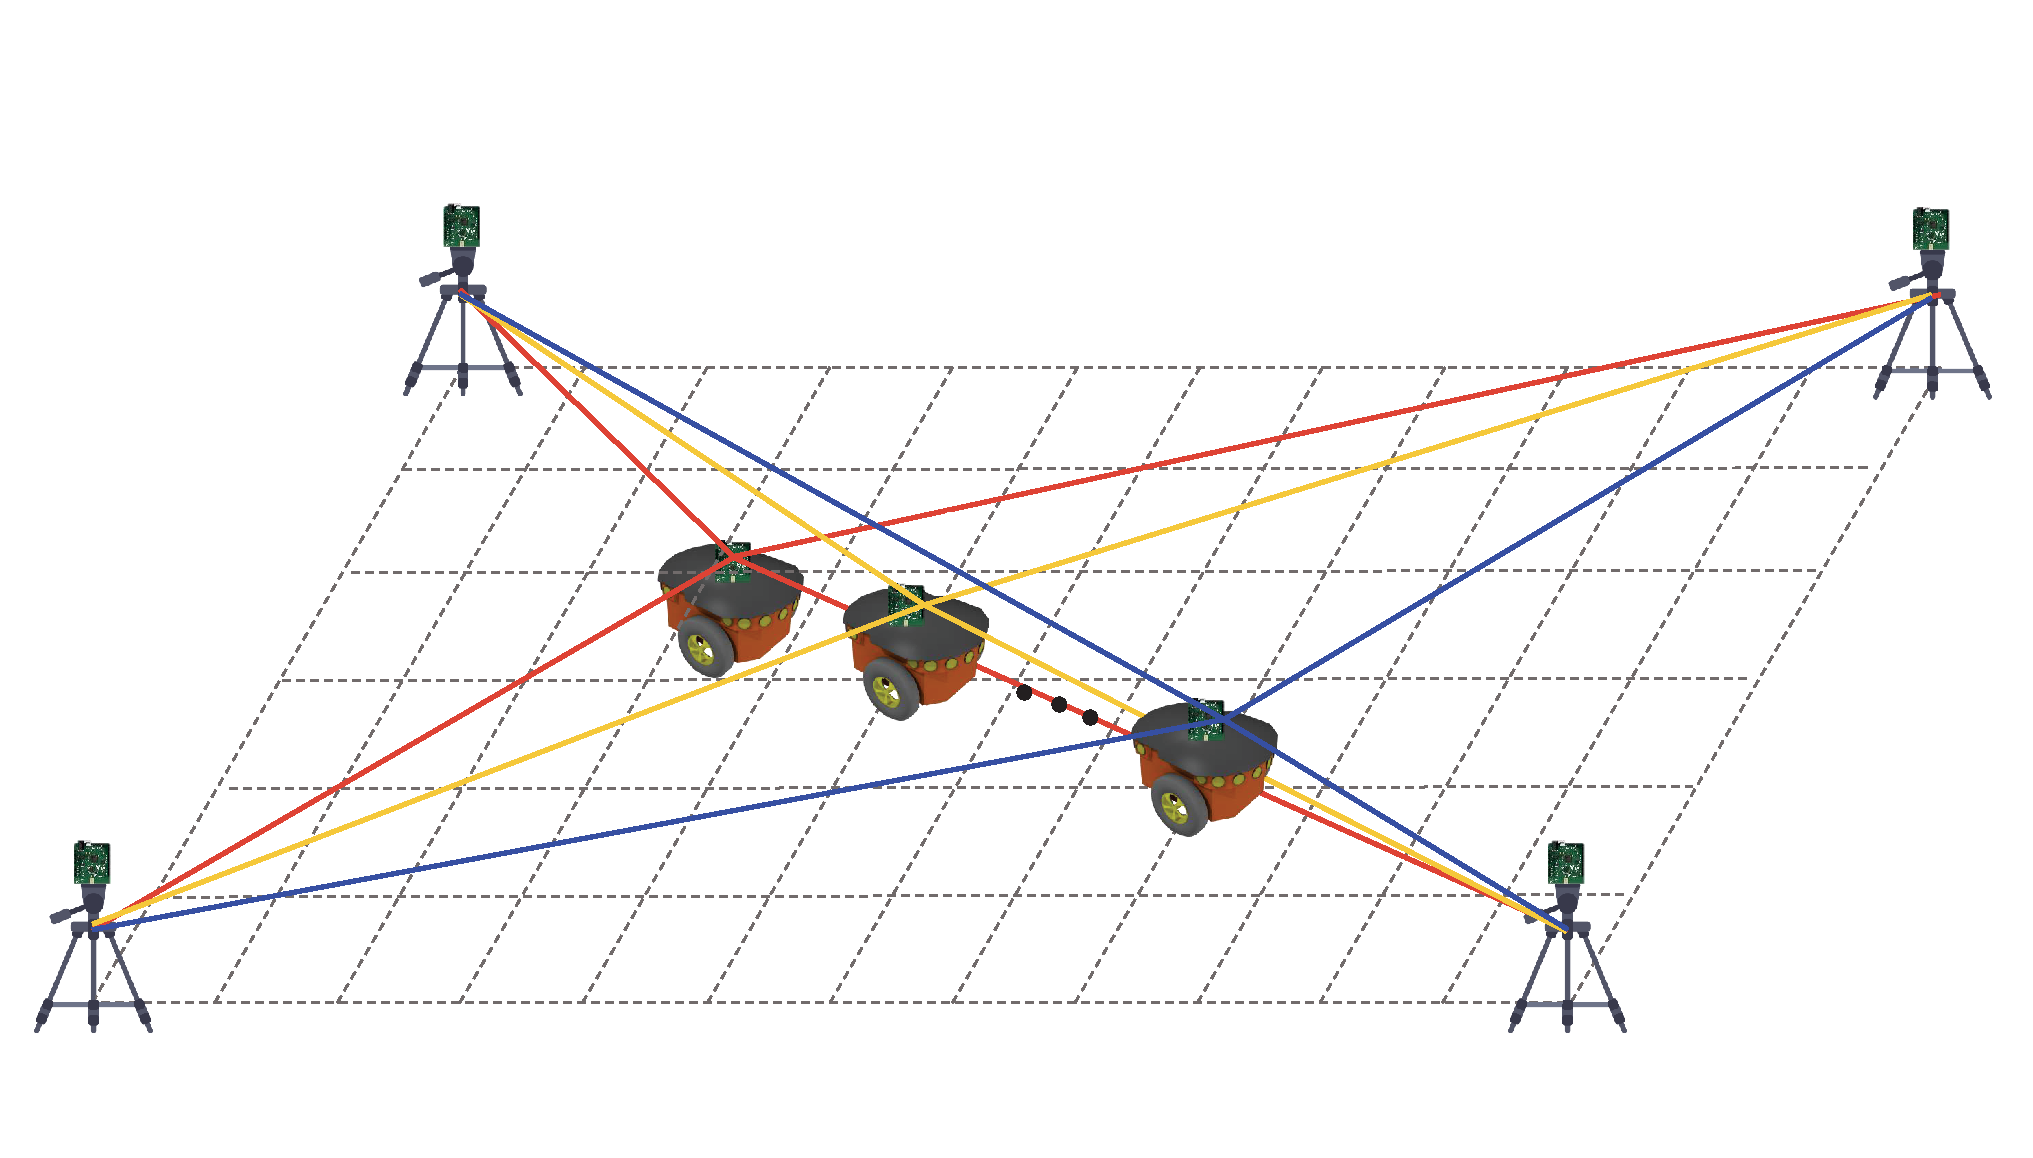
\includegraphics[height=4.5cm]{IROS2018_image_1}
	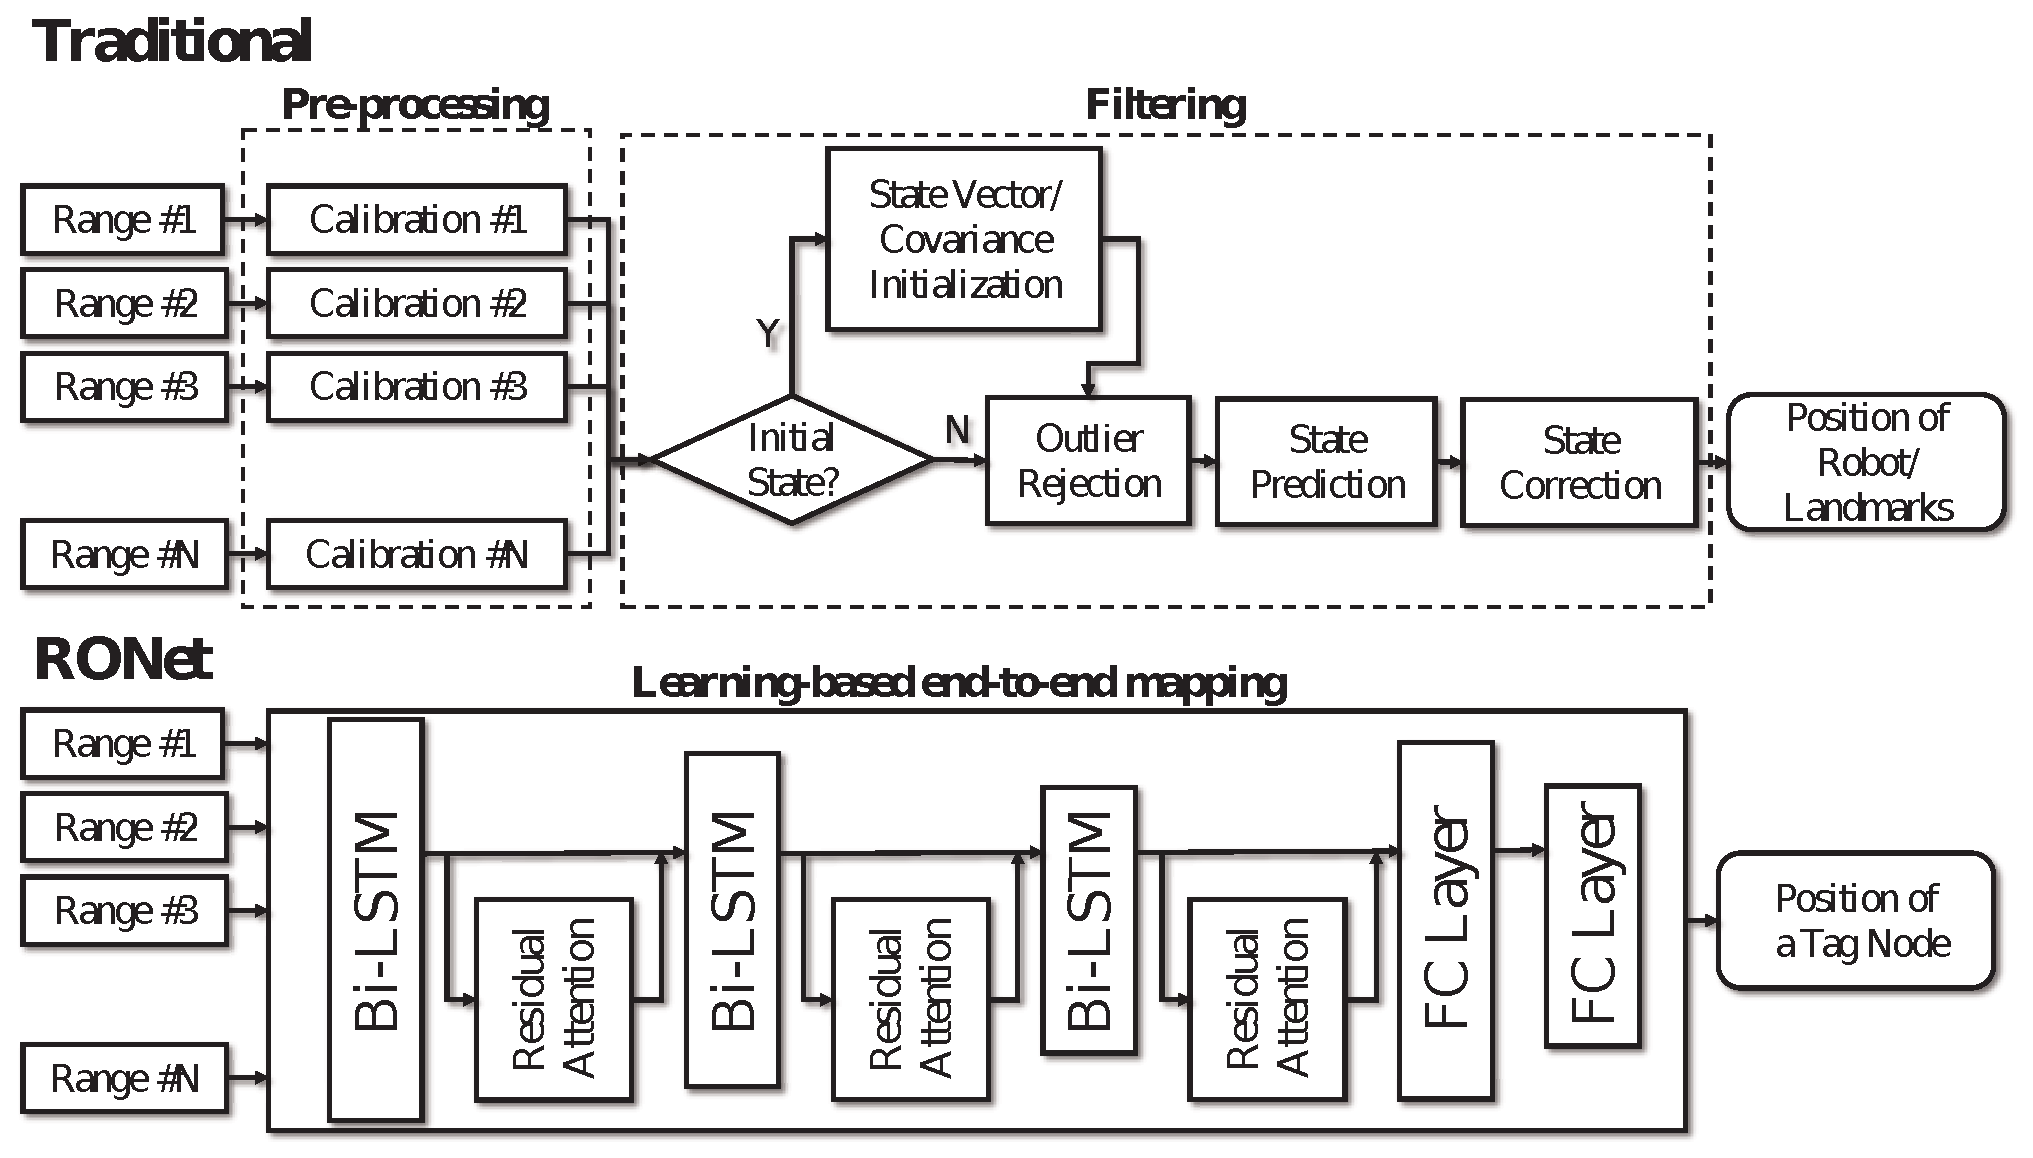
\includegraphics[height=5cm]{image/conventional_deep_v2}
	
	%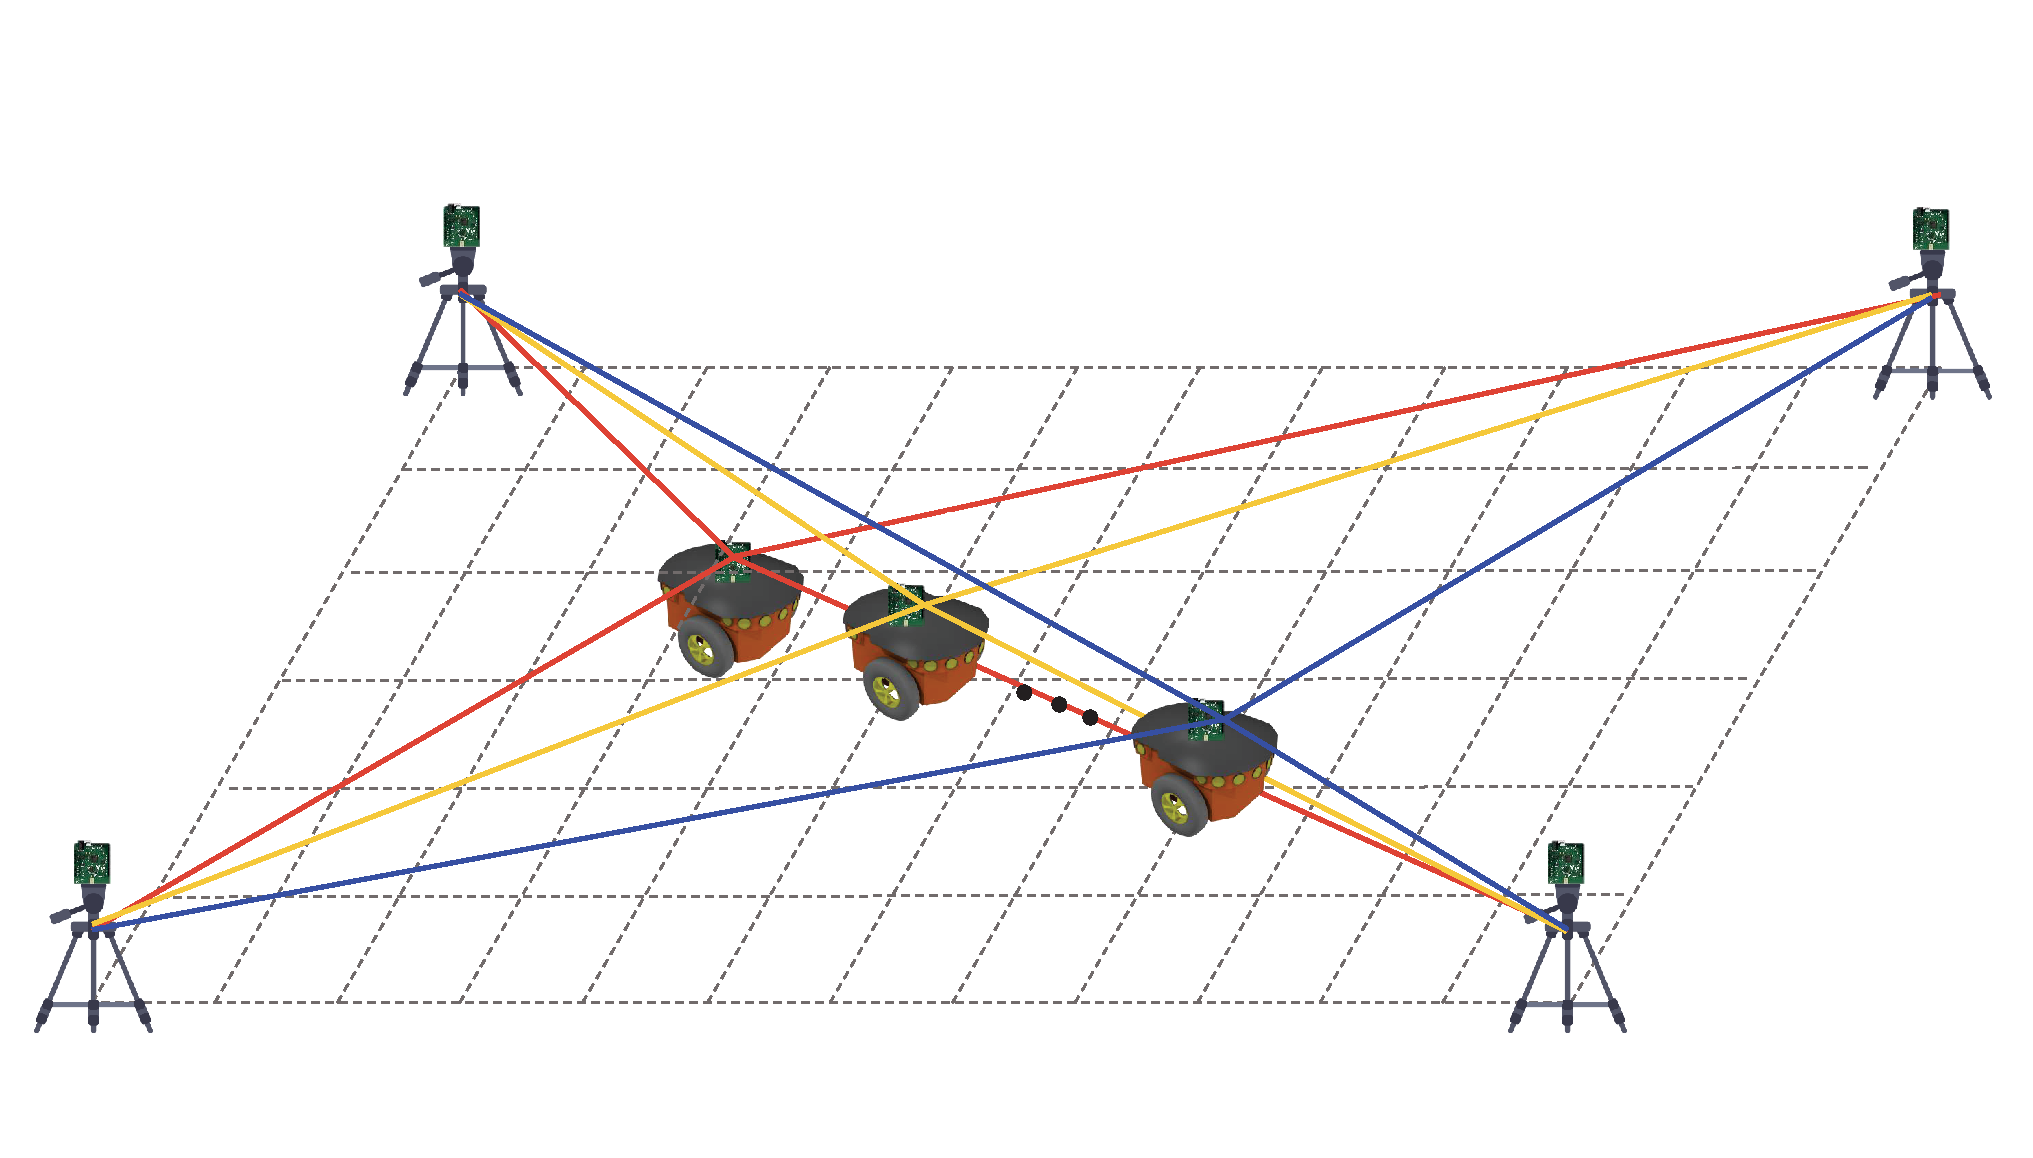
\includegraphics[trim={0 0 0 1cm}height=4.5cm]{IROS2018_image_1}
	\label{fig:overview}
	%	}
	
	\caption{Comparison between a conventional probabilistic-based range-only framework and our learning-based approach.}
	
\end{figure}

To alleviate these issues, many studies have been conducted based on probabilistic Bayesian inference frameworks and Monte-Carlo Bayesian filters. However, in recent years, numerous attempts have been extended to solve these problems based on neural network-based approaches \cite{rahman2009localization, abdelhadi2013efficient, kumar2016localization, lim2018effective}. With nonlinear end-to-end mapping, prior studies showed feasibility. However, in most cases, researchers only utilized multilayer perceptrons (MLP) that constitute the front-end architecture in deep learning fields \cite{rahman2009localization, abdelhadi2013efficient, kumar2016localization}. In \cite{lim2018effective}, a stacked bidirectional long short-term memory (Bi--LSTM) layer was implemented to account for the noise of range observations based on the network’s characteristics that accepted temporal sequential values as input. However, they only tested this formulation in a simulated environment\cite{rahman2009localization, abdelhadi2013efficient, kumar2016localization}. Additionally, none of the prior studies investigated whether their learning-based approaches could be executed in real time or not. 

In this study, we propose a robust stacked Bi--LSTM network with residual attention, named as RONet. To the best of our knowledge, it is the first approach that applies an LSTM-based architecture to localize a mobile robot in real time using only range measurements in realistic environments. Unlike conventional probabilistic-based algorithms, it does not need any preprocessing modules, such as calibration, or outlier rejection. Besides, RONet yields better and more precise performance and results in increased robustness against outliers compared to the conventional range-only approach based on a particle filtering and the use of deep learning-based approaches.

Our contribution is threefold:
\begin{itemize}
	%\setlength{\itemindent}{-.5in}
	\item Three-stacked Bi--LSTM layers on which residual attention layers are attached are proposed to allow the neural network to be trained well so that the RONet yields the best performance compared to previous approaches.
	\item We also analyze how the sequential length of the network affects performance and evaluate the robustness of the RONet with a minimum number of anchors.
	\item We operate the RONet on Nvidia Jetson AGX Xavier and confirm whether the inference frequency (which is approximately 32 Hz) complies with real-time. 
\end{itemize}

The rest of the study is organized as follows: Section II overviews related, previously published studies. Section III defines the problem to be solved and describes our neural network in detail, and Section IV describes the experimental results. Finally, Section V summarizes our contributions and describes future work.

\section{Related Works}
\subsection{Conventional Range-Only Localization}

There are two conventional approaches to localize a mobile robot using range measurements: methods based on a) Kalman filtering (KF) or b) particle filtering (PF). However, unlike other sensors, it is difficult to approximate range measurements using linear models owing to MPF or non-line-of-sight issues (NLOS). Thus, some authors insisted that PF-based approaches could be better than KF-based approaches because PF can cope with complex nonlinear models and also cover multimodal distributions \cite{gonzalez2009mobile, blanco2008pure, shetty2018particle}. 

Fig. 1 shows the general steps used by the conventional probabilistic approaches. First, each range of measurements needs to be calibrated. After initialization, the algorithm checks whether an input value is an outlier or not, and then eliminates unexpectedly large noise values. Subsequently, it predicts the present states, including the mobile robot's pose and anchor locations, and finally, it corrects its prediction using range observations.

 \begin{figure*}[h]
	\centering
	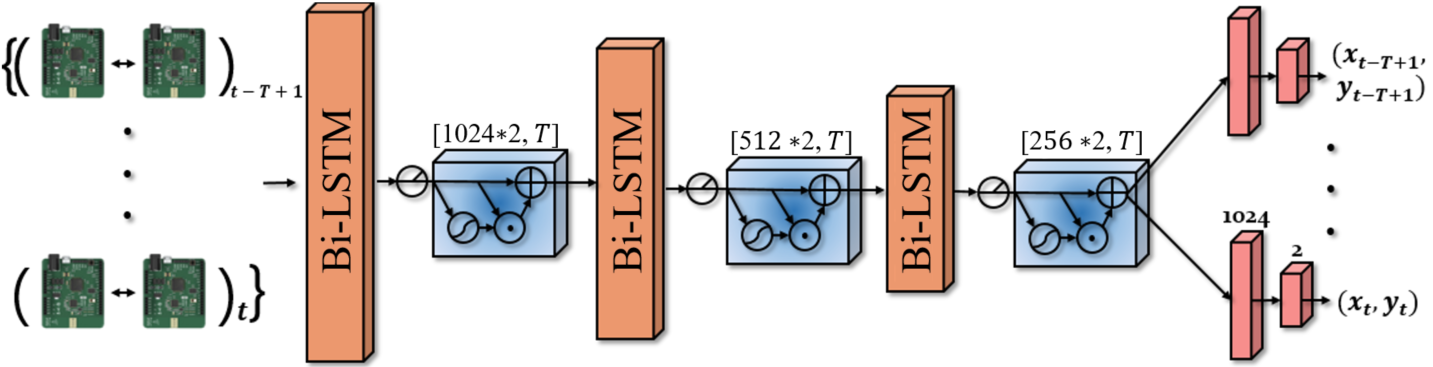
\includegraphics[width=0.95\linewidth]{image/network_figure}
	\caption{Our networks consist of three elements: a) Bi--LSTM, b) the residual attention module (the blue cuboid), and c) the fully connected layer (FC layer). Features are input to the Bi--LSTM, which reduces the number of features in half from 2048 to 1024 to 512. Finally, extracted features are input to the FC layer to estimate the position corresponding to each time step.}
	\label{fig:our_network} 	
\end{figure*}

\subsection{LSTM-based Sequential Modeling}

In view of the rapid development of deep learning approaches \cite{lecun2015deep}, various types of deep neural architectures have been proposed for localization tasks \cite{kendall2016modelling, kendall2015posenet, gladh2016deep}. Specifically, recurrent neural networks (RNNs) that originated from the natural language process (NLP) area \cite{elman1990finding} have been shown to achieve better performance in cases associated with time-variant information. 

Additionally, despite the fact that long short-term memory (LSTM) architecture solves the \textit{long-term dependency} issue that is inherent to RNNs, it is unable to learn the relationship of sequential information as the time-sequential gap grows \cite{hochreiter1997long}. Accordingly, LSTM is actively introduced to learn longer-term contextual understandings. Therefore, many researchers exploited LSTM for sequential modeling after feature extraction by Convolutional Neural Networks (CNN) \cite{clark2017vinet,patel2018contextualnet, wang2017deepvo}. 

 
\subsection{Deep Learning for Range Only Localization}

LSTM is also utilized to model low-dimensional sensor data by itself. In \cite{wang2018deepml}, they exploited LSTM for indoor localization with magnetic and light sensors. In \cite{chen2018ionet}, they estimated two-dimensional (2D) odometries via stacked Bi--LSTM that utilized Inertial Measurement Unit (IMU) sensor data only as input. 

Regarding our objective for localization using range-only measurements, we note that many researchers had previously employed neural network-based approaches in wireless sensor networks fields (WSNs) \cite{rahman2009localization, abdelhadi2013efficient, kumar2016localization}, yet most networks had been based on the MLP. Their approaches only mapped a set of range observations without temporal context to achieve localization. Accordingly, their approaches may be more potentially week to unexpected noise that is not included in the train data. Another study \cite{lim2018effective} implemented stacked Bi--LSTM for localization of a mobile robot that obtained sequential range measurements from anchors and tags. However, the researchers conducted only simulations in which there were no MPFs or unexpected noise. Therefore, in this study, we conducted realistic experiments to verify the feasibility of the approaches to account for all the noise sources from all sensors with sequential range information followed by the comparison of these approaches.

\subsection{Attention Layer}

An attention layer is a powerful module nowadays and mostly improves the performance of a neural network. Originally, neural networks treat information equally. However, using attention layers, some parts of the neural networks can be examined more closely. Accordingly, the attention layer plays the role of a feature selector \cite{wang2017residual}. Initially, attention was utilized at the NLP areas for the improvement of the translation performance \cite{luong2015effective}. Nowadays, however, the attention layer is employed in many areas to improve the performance of the networks. 

\section{RONet}

In this section, our proposed residual attention-based stacked Bi--LSTM will be explained, as illustrated in Fig. \ref{fig:our_network}. 
Specifically, we introduce the stacked Bi--LSTM and residual attention module for localizing the tag node, and the outcomes are compared to those from other previous publications. Finally, the way how to set the loss function of our neural network will be described. 

\subsection{Long Short-Term Memory}

Unlike the RNN that only consists of a hidden state, in LSTM, a cell state is added to the network\cite{hochreiter1997long}. The cell state consists of three gates to preserve the previous information and control the cell state, i.e., a) forget, b) input, and c) output gates. The respective equations of these gates are as follows:

\begin{align}
f_{t} & =\sigma _{s}\big(W_{xf}\cdot x_{t}+W_{hf}\cdot h_{t-1}+b_{f}\big)\label{eq:forget}\\
i_{t} & =\sigma _{s}\big(W_{xi}\cdot x_{t}+W_{hi}\cdot h_{t-1}+b_{i}\big)\label{eq:input}\\
\tilde{c}_{t} & = \tanh\big(W_{xc}\cdot x_{t}+W_{hc}\cdot h_{t-1}+b_{c}\big)\label{eq:new_cell}\\
c_{t} & =f_{t}\odot c_{t-1}+i_{t}\odot\tilde{c}_{t}\label{eq:update}\\
o_{t} & =\sigma _{s}\big(W_{xo}\cdot x_{t}+W_{ho}\cdot h_{t-1}+b_{o}\big)\label{eq:output}\\
h_{t} & =o_{t}\odot \tanh\big(c_{t}\big)\label{eq:hidden}
\end{align}
where $\sigma _{s}$ is an activation function, known as \textit{sigmoid}, $f_{t}$, $i_{t}$, $o_{t}$, respectively denoting the forget, input, and output gates. $c_{t}$ and $h_{t}$ denote the cell state and the hidden state. $\odot$ denotes element-wise multiplication, referred to as the \textit{Hadamard product}. All the gates are activated by the sigmoid function and the cell states are activated by the $\tanh$ function.

The forget gate layer, $f_{t}$, determines how much information to forget based on the previous hidden state, $h_{t-1}$, and the present input, $x_{t}$. Subsequently, the input gate, $i_{t}$, decides how much information to include when the cell state is updated. Accordingly, in \eqref{eq:update}, $c_{t}$ is updated by the cell state layer based on $f_{t}$, $i_{t}$, and by the candidate cell state, $\tilde{c}_{t}$. In addition, in \eqref{eq:output}, the output gate layer, $o_{t}$, serves as a filter, which means that $o_{t}$ determines the values which will be output in such a way that $h_{t}$ is updated based on the updated cell state of $o_{t}$ and $c_{t}$ in \eqref{eq:hidden}. 

\subsection{Stacked Bidirectional LSTM}

\begin{figure}[h!]
	\centering
	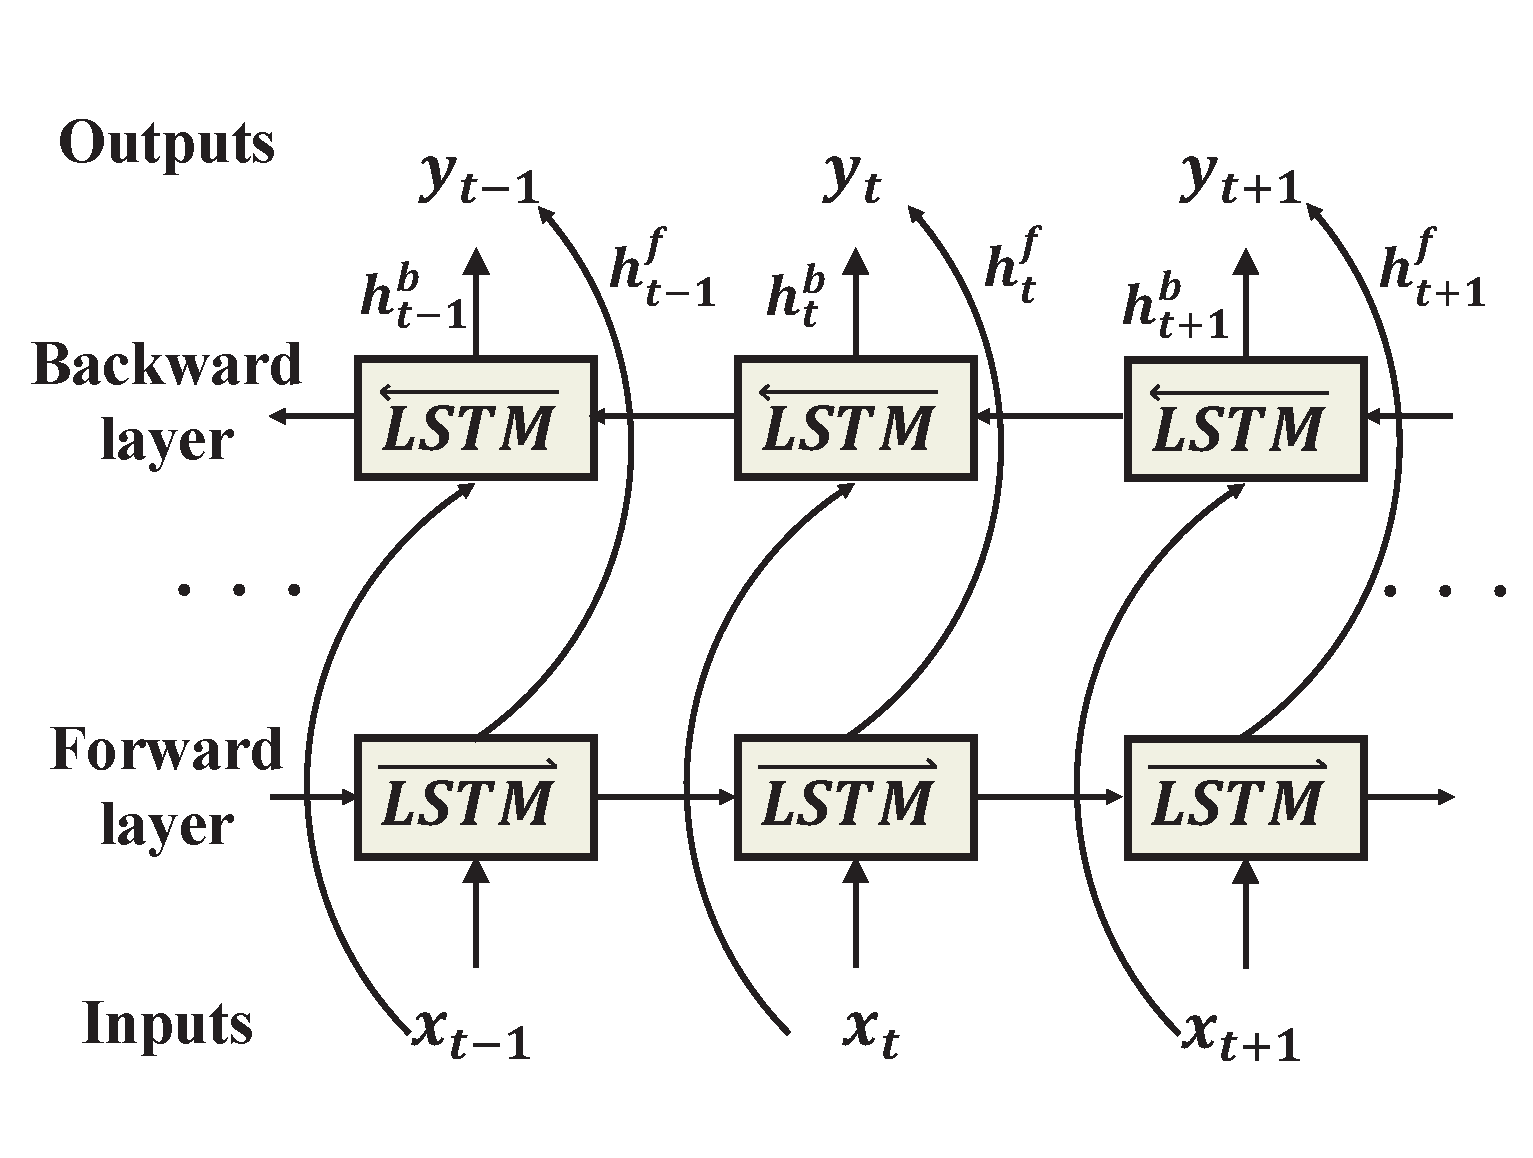
\includegraphics[width=.9\linewidth]{image/bidirectional_LSTM}
	\caption{The architecture of the bidirectional LSTM (Bi--LSTM). The bidirectional LSTM consists of two LSTMs: one forward (right arrow) and one backward (left arrow) LSTM layer.}
	
	%$\overrightarrow{LSTM}$, and one backward LSTM layer, $\overleftarrow{LSTM}$}
	\label{fig:bidirectional_revised}	
\end{figure}

Based on the fact that the deeper the architectures of the neural networks are, the better their performances \cite{simonyan2014very, he2016deep}, many researchers have analyzed variations of LSTM architectures and found that stacking multiple LSTM layers improves the performance for many tasks \cite{graves2013hybrid, graves2013speech, ullah2018action}. Furthermore, bidirectional RNNs are introduced \cite{schuster1997bidirectional} to extract well-described contexts. They consist of one forward LSTM, $\overrightarrow{LSTM}$, and one backward LSTM, $\overleftarrow{LSTM}$, running in reverse time so that the network exploits the previous forward context to update $h_{t}$ and $c_{t}$, and the future backward context as well, as shown in Fig. \ref{fig:bidirectional_revised}. 

For these reasons, we decided to implement the stacked Bi--LSTM architecture to model the system. By virtue of the increased nonlinearity caused by the number of stacked layers, the network could model more complex localization schemes by considering the UWB-ranging observations as the input that contain unexpected noise and MPF problems. Furthermore, we determined that Bi--LSTM would be more helpful in the production of more appropriate context by concurrently considering both the past and the future.

Therefore, we constructed our networks by stacking three Bi--LSTM networks to increase the nonlinearity. Note that simply stacking more than three LSTM layers does not result in additional performance improvements and become hard to be trained well. It is caused by the \textit{vanishing and exploding gradient problem} \cite{hochreiter2001gradient, pascanu2013difficulty,pascanu2012understanding} according to which the networks fail to perform training owing to the fact that the gradient is getting closer to zero or explodes out of prefixed memory during the backpropagation. Consequently, the Rectified Linear Unit (ReLu) function is placed between the LSTMs \cite{nair2010rectified} instead of stacking more LSTM layers to increase nonlinearity. In addition, experiments showed that reducing the hidden size of the next LSTM layer when the features are input into the LSTM layer slightly increases performance. In conclusion, we decided to set the respective sizes of the three layers to 1024, 512, and 128. Note that when adopting the Bi--LSTM, the actual feature sizes were set to 2048, 1024, and 256, respectively. At the end part of the LSTM, fully connected layers were attached to predict the position of the mobile robot based on the sequential features processed by the LSTMs.  

\subsection{Residual Attention Layer}

To precisely estimate the position of the tag node, it is important for the network to distinguish the most meaningful context based on the time step \textit{T} to help contextual understanding of our networks. The equation of the original attention mechanism is as follows:   

\begin{equation}
H(x)=M(x)\odot x
\end{equation} 
where $x$ denotes the output of the previous neural network layer, $H(x)$ denotes the output of the attention layer to be forwarded to the next neural network layer, and $M(x)$ denotes the attention mask. Based on the multiplication of $x$ by $M(x)$ in an element-wise manner, the network weight established by the attention layer represents crucial information. 

Despite the improvement of the performance, the attention layer is associated with potential risks in that it may dilute the features because the attention mask value ranges from zero to one. Thus, we adopted a residual attention layer to alleviate this problem as follows \cite{wang2017residual}:

\begin{equation}
H(x)=\left(1+M(x)\right)\odot x.
\end{equation} 

As shown by the blue cuboid shape in Fig. \ref{fig:our_network}, this idea is originated from ResNet \cite{he2016deep} that contains skip connections in such a way so as to mitigate the aforementioned dilution problem and help the network to be properly trained. Similar to the ResNet, residual attention also contains other branches which are used to calculate how much attention is required. These branches are joined by the original feature vectors $x$. Each hidden state consists of a residual attention layer so that these attention modules can a) determine which time stamp is more meaningful and b) deliver the output to the next bidirectional LSTM.

\subsection{Training Loss}

In this subsection, the method for training our network is described. Let $n$ be the number of anchor nodes of the dataset, $L_{t}$, containing the measured values of each anchor node, tag node; and ground truth of the 2D positions, $Y_t$, be represented at each time step $t$ as follows: 

\begin{equation}
L_{t} = (l_{1}, l_{2}, ..., l_{n})_{t}
\end{equation}
\begin{equation}
Y_t = (x_t, y_t)
\end{equation}
where $l_{i}$ denotes the distance between the $i$-th anchor and tag nodes. Note that our neural network does not only accept a set at time $t$ but also accepts sets based on the sequential length, $T$, of input to the network, $\mathbb{L}_t$, as follows:

\begin{equation}
%$L = \left\{(X_t, Y_t)\right \}$ 
\mathbb{L}_t = \left\{L_{t-T+1}, L_{t-T+2}, ..., L_t\right\} 
\end{equation}
\begin{equation}
\mathbb{Y}_t = \left\{Y_{t-T+1}, Y_{t-T+2}, ..., Y_t\right\}.
\end{equation}

Consequently, neural networks could be optimized to be able to localize the mobile node by being trained using the training dataset $\mathbb{D}$ as follows:  

\begin{equation}
%$L = \left\{(X_t, Y_t)\right \}$ 
\mathbb{D} = \left\{(\mathbb{L}_{T-1}, \mathbb{Y}_{T-1}),...,(\mathbb{L}_t, \mathbb{Y}_t),...\right\}.
\end{equation}

Therefore, let $\Theta$ be the parameters of our network model. Our final goal is to find optimal parameters $\Theta^{*}$ for precise localization by minimizing the $L_2$ loss term. The $L_2$ loss term denotes the mean-square-error (MSE) of the Euclidean distance between the normalized ground truth position $\mathfrak{N}(Y_k)$ and the estimated position $\hat{Y_k}$, as follows:

\begin{equation}
\Theta^{*} = \underset{\Theta}{\mathrm{argmin}} \frac{1}{N}\frac{1}{T} \sum_{k=T-1}^N\sum_{m=k-T+1}^k \parallel \mathfrak{N}(Y_m) - \hat{Y_m} \parallel^{2}.
\end{equation}  

\begin{figure*}[h]
	\centering
	\begin{subfigure}[b]{0.32\textwidth}
		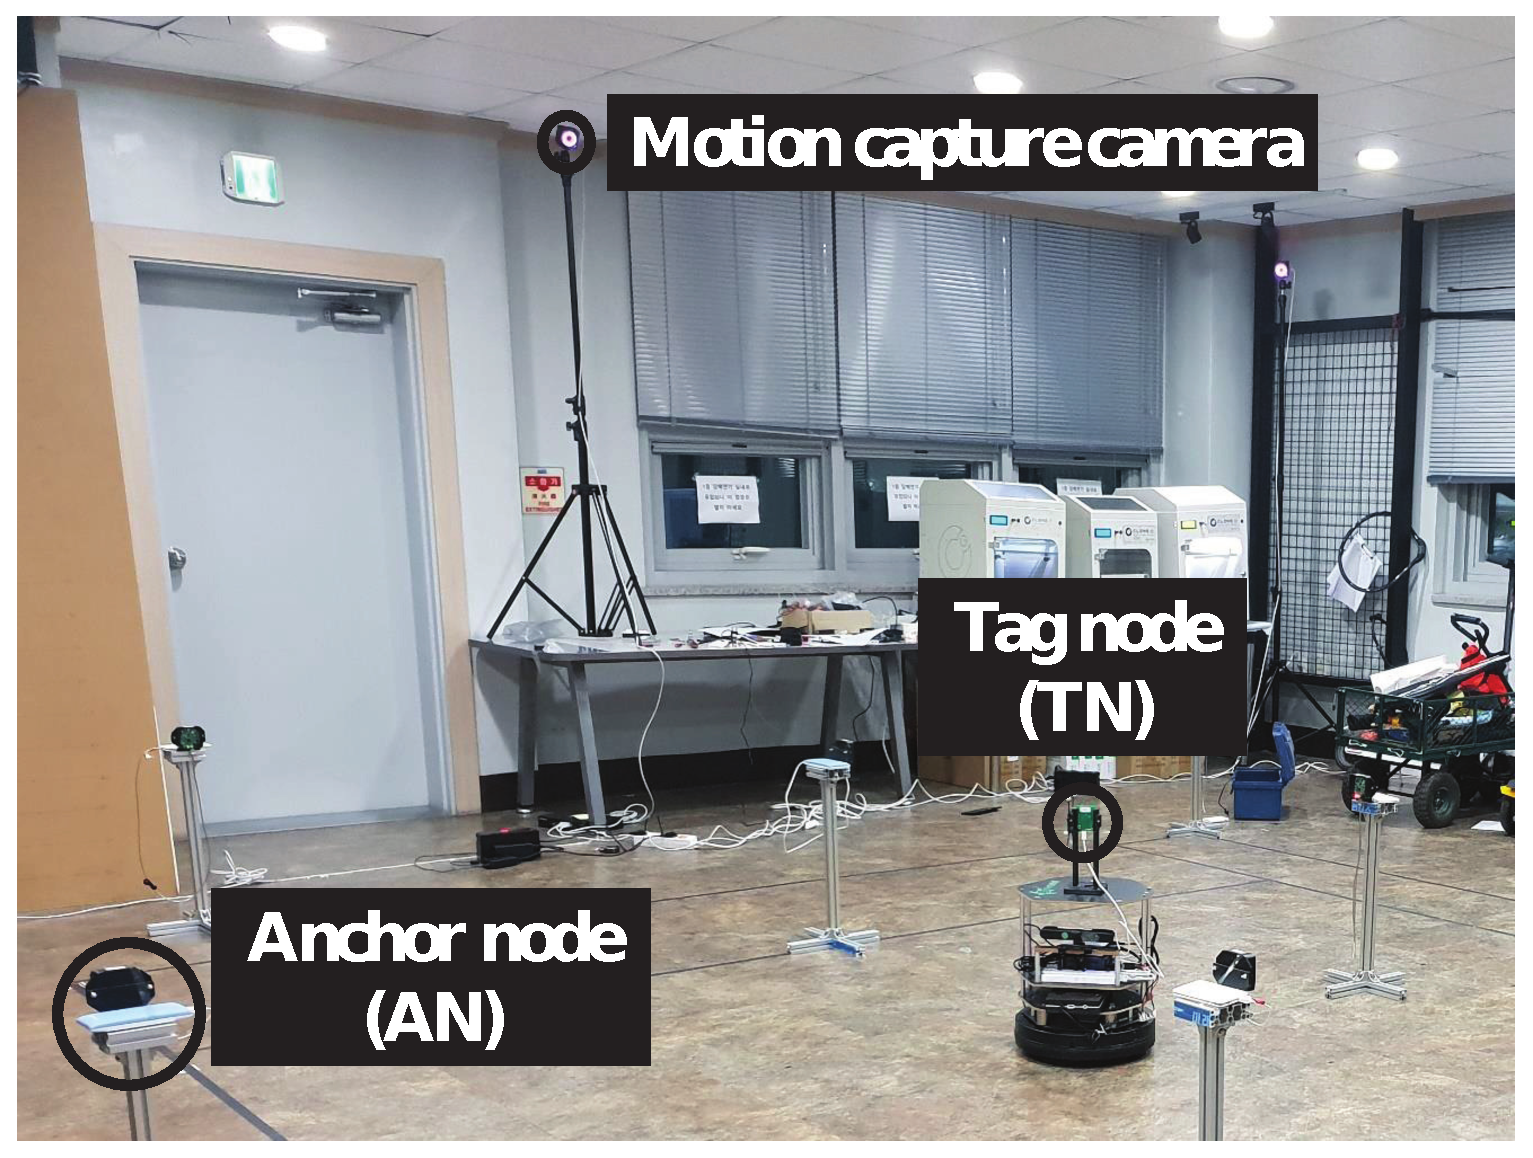
\includegraphics[width=\textwidth]{image/system_whole_picture}
		\caption{}
		\label{fig:whole_system}
	\end{subfigure}
	%add desired spacing between images, e. g. ~, \quad, \qquad, \hfill etc. 
	%(or a blank line to force the subfigure onto a new line)
	\begin{subfigure}[b]{0.32\textwidth}
		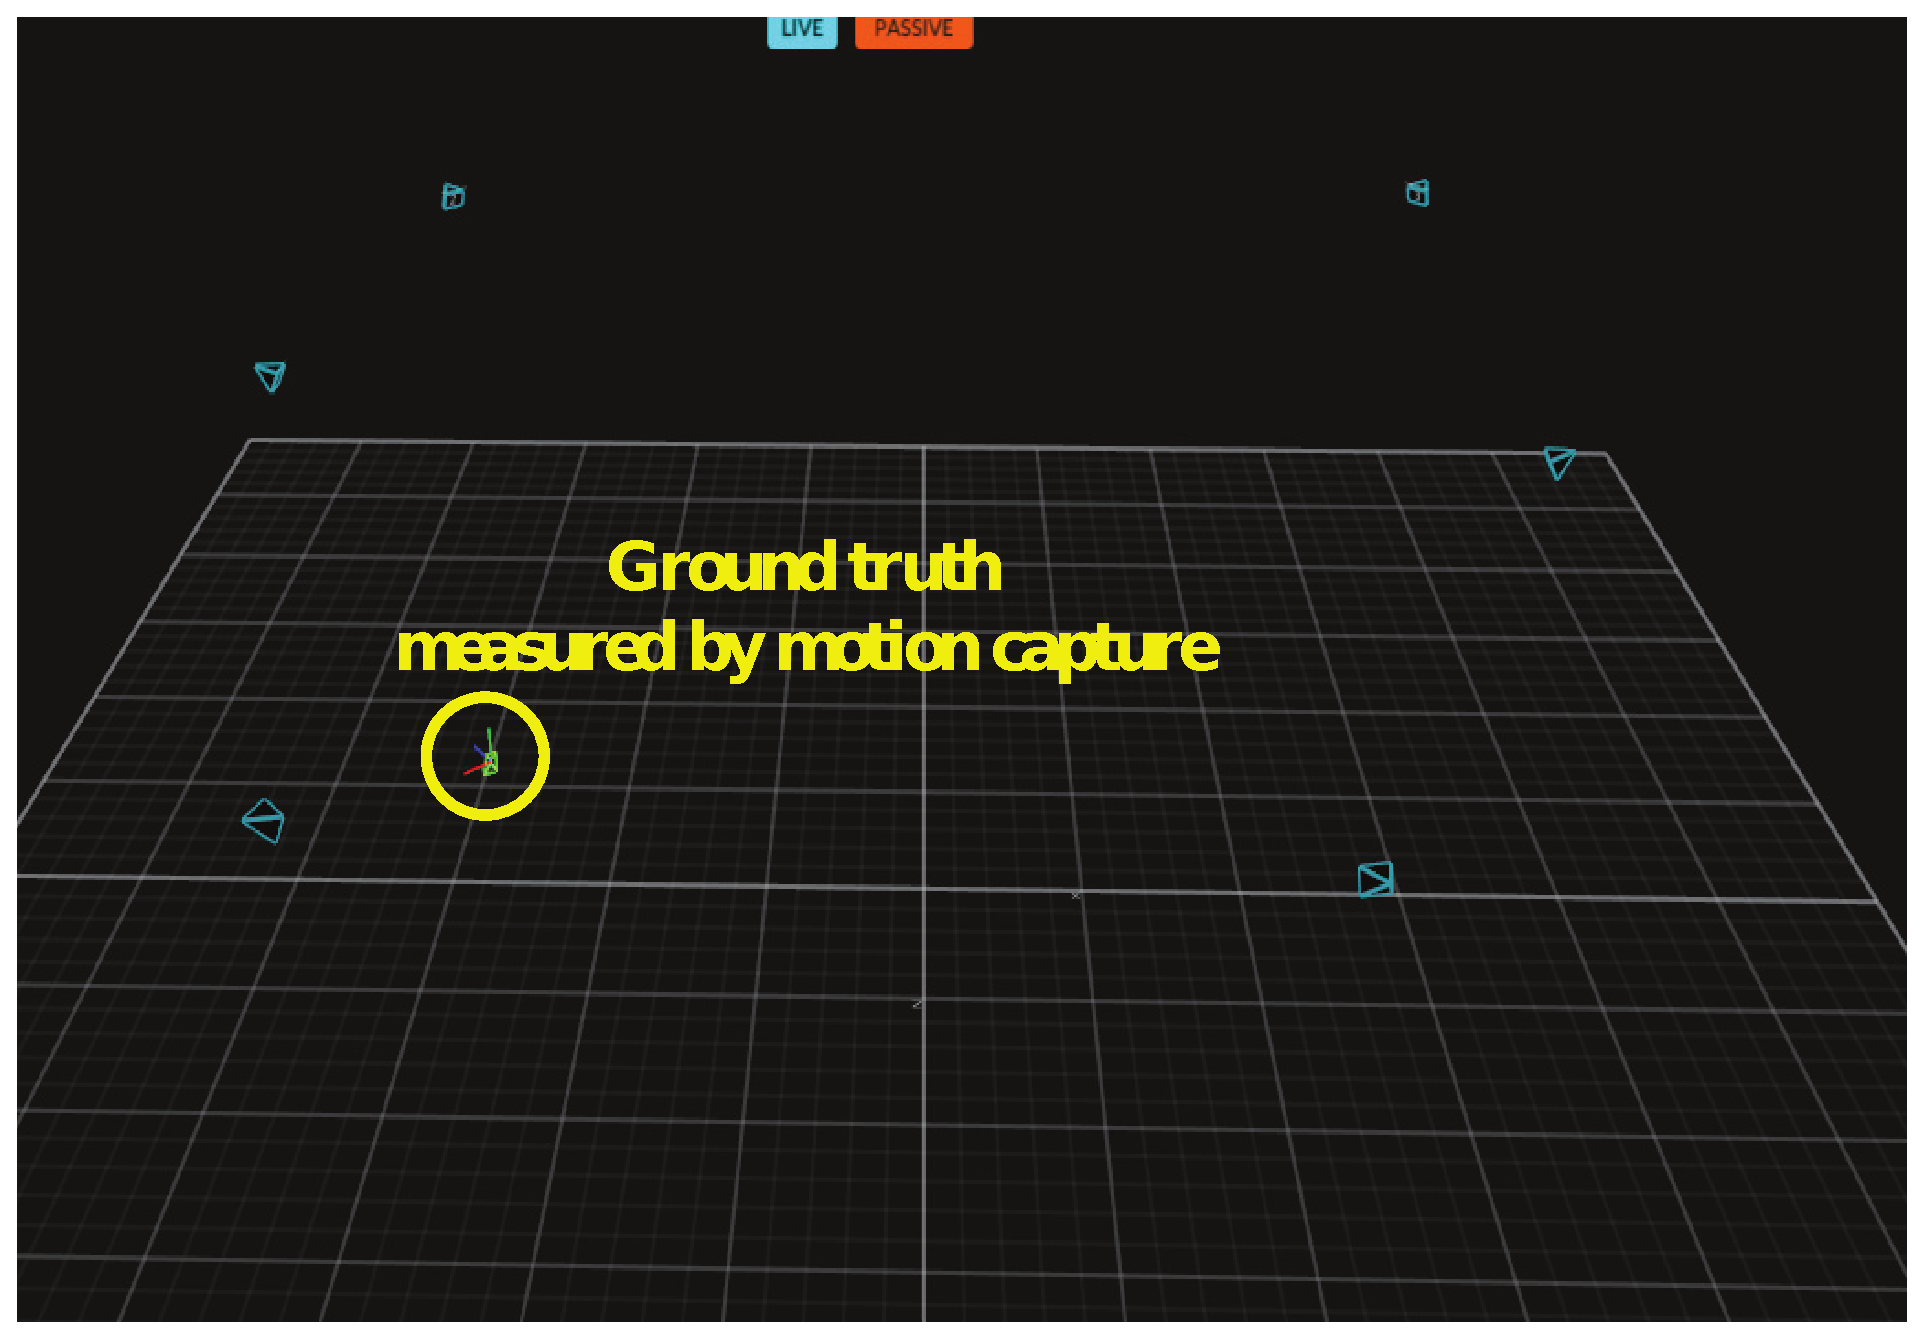
\includegraphics[width=\textwidth]{image/motion_capture}
		\caption{}
		\label{fig:Optitrack_figure}
	\end{subfigure}
	%add desired spacing between images, e. g. ~, \quad, \qquad, \hfill etc. 
	%(or a blank line to force the subfigure onto a new line)
	\begin{subfigure}[b]{0.32\textwidth}
		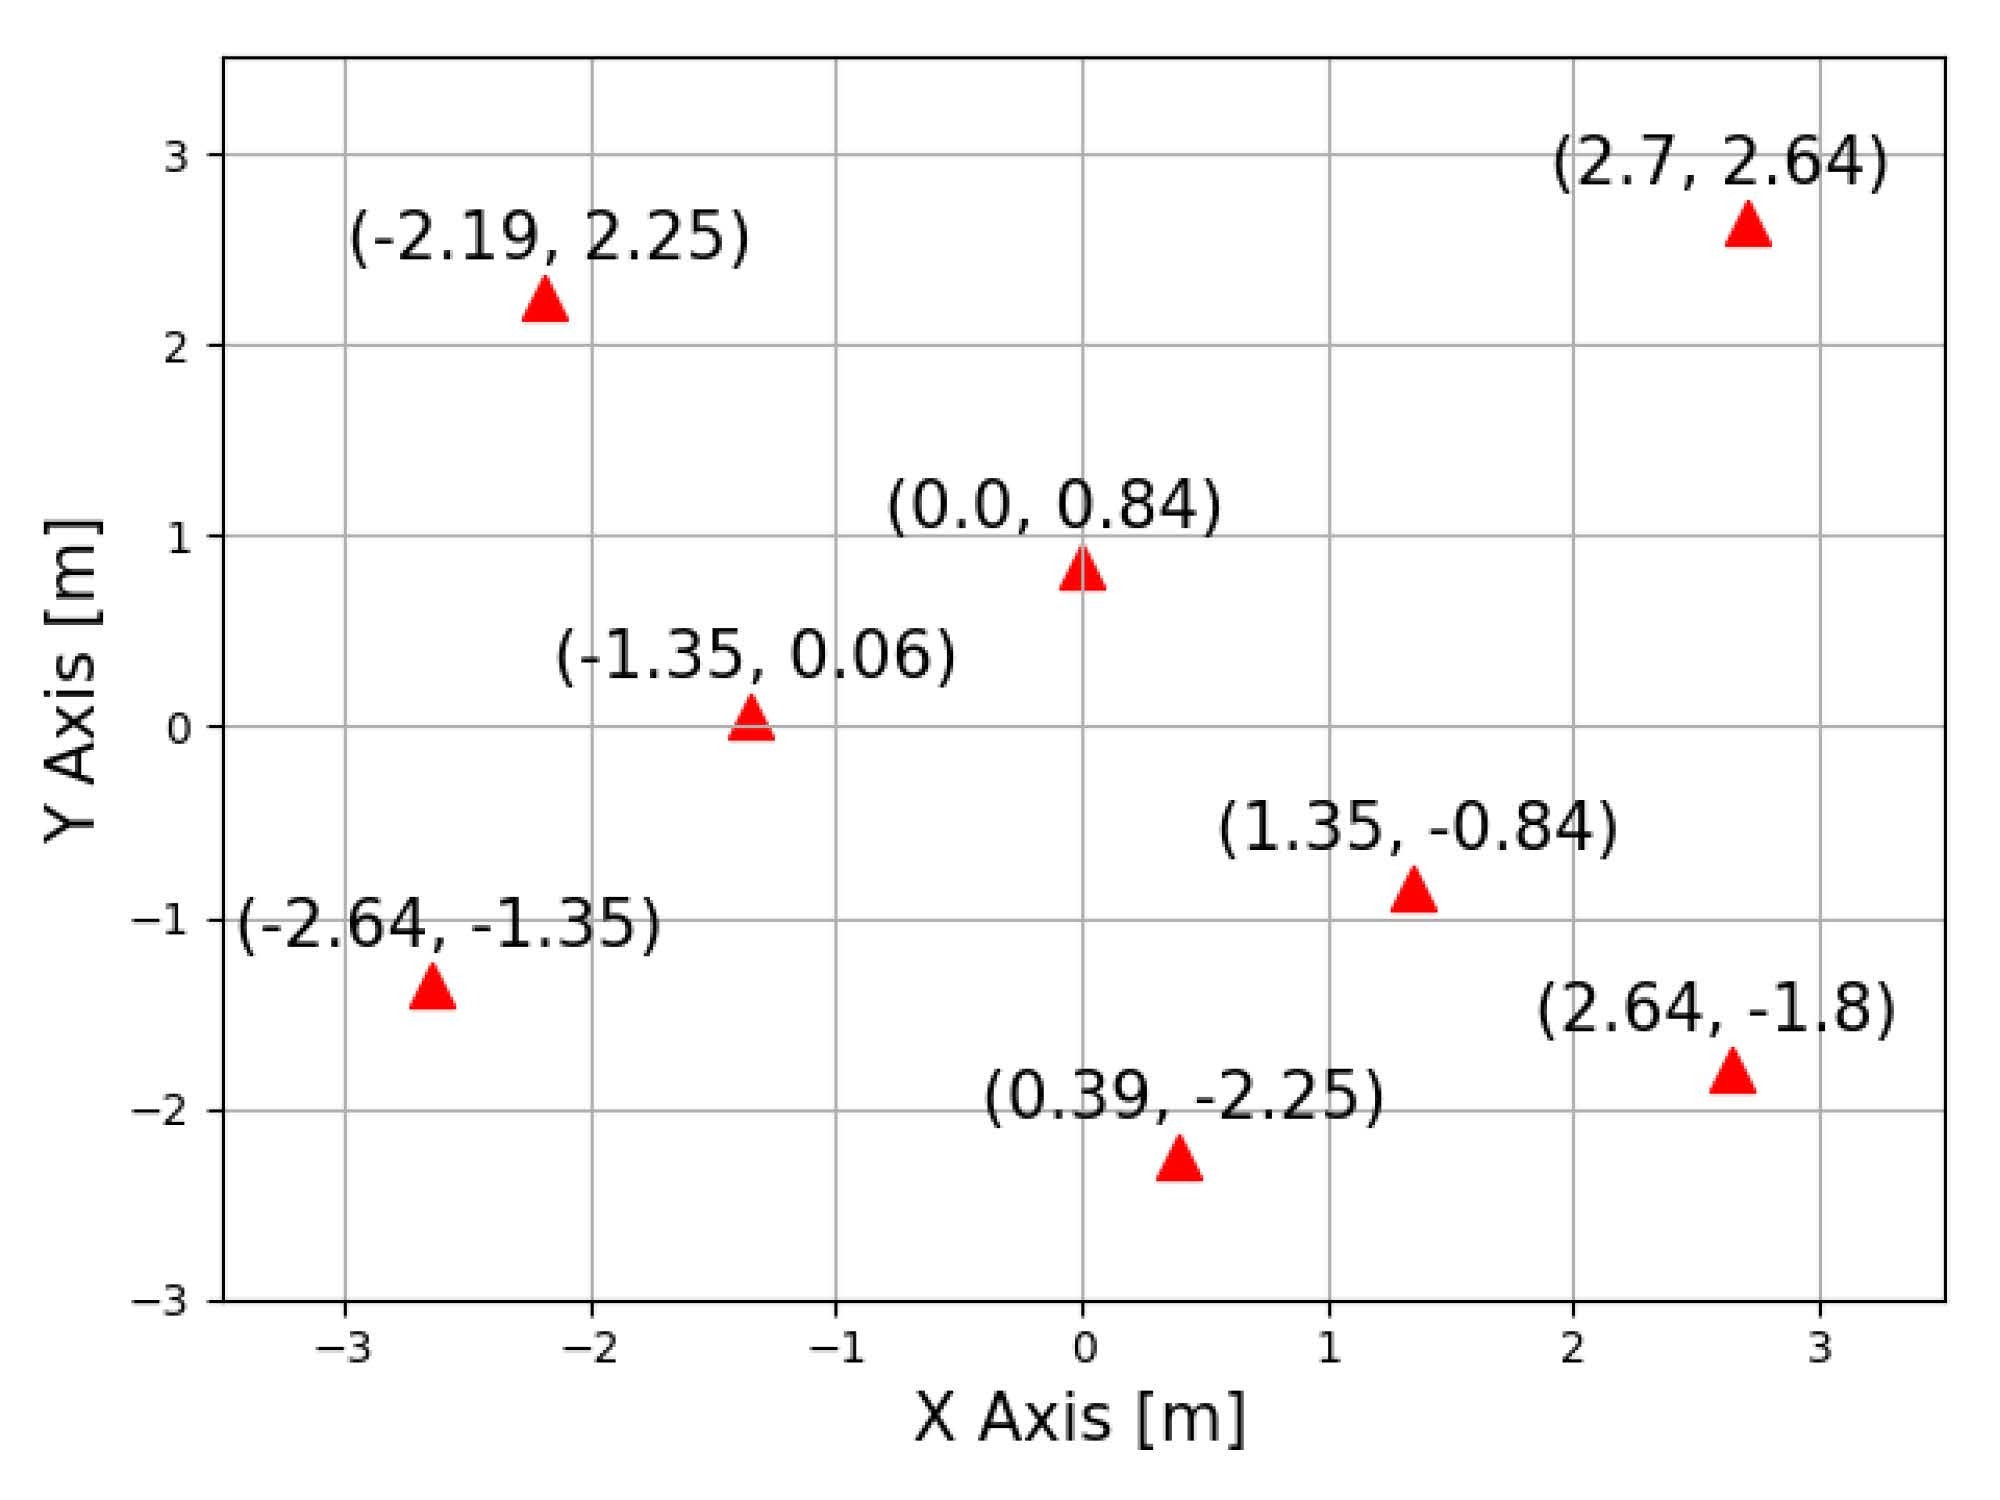
\includegraphics[width=\textwidth]{image/system_exact_position}
		\caption{}
		\label{fig:Exact_position}
	\end{subfigure}
	\caption{(a) Experimental environment. (b) Tracked pose from Optitrack motion capture. (c) Exact position of anchor nodes. }\label{fig:experimental_envorinment}
\end{figure*}

\section{Experimental Results and Discussion}
\subsection{Experimental Environment}

Our experimental system consists of an Ultra-Wide Band (UWB) sensor tag node attached on the mobile robot platform and eight anchor nodes that act as UWB transceivers. There are six Optitrack Prime 13 motion capture cameras for ground truth position measurement. We utilized an Nvidia Jetson AGX Xavier Developer Kit\cite{xavier2018}, which is a small-form-factor (SFF) computer that has a 512-core Volta graphics processing unit (GPU) with Tensor Cores. Fig. 4(a)
 shows our experimental environment and indicates how the anchor and tag nodes are attached. In addition, we used the mobile platform TurtleBot2 from Yujinrobot\cite{turtlebot22013}.

The tag node receives the signal and measures the range between two devices based on the time-of-flight (TOF) and the received signal strength indication (RSSI). UWB transceivers consist of a Pozyx developer tag and Pozyx anchors\cite{pozyx2018}, comprising a DW1000 UWB-chip made by Decawave. The measurement accuracies are at the cm level.
 
\subsection{Acquisition of the Train/Test Data}

UWB sensor anchors are installed randomly in the region where motion capture cameras are receptive, as Fig. 4(c)
 shown. These anchor nodes transmit the UWB signal to a tag node that is attached to the mobile robot, while the Optitrack motion cameras also transmit the ground truth data to the SSF computer by utilizing the Robot Operating System (ROS).

Note that these two datasets are transmitted at different frequencies: range measurements were obtained at a frequency of about 27 Hz, yet the ground truth data were obtained at 120 Hz. Thus, we synchronized these two data based on the range measurements. Specifically, we set an independent thread so that it a) selected the ground truth data of the closest time instant based on the UWB range measurements, b) concatenated, and c) saved these data.

Moreover, the mobile robot moved within this space controlled by a keyboard manually. All the trajectories are thus different. After collecting complete datasets, we separated the entire dataset into three types: one of them to the training dataset, another to the validation dataset, and the rest to the test dataset. In the case of the test dataset, only range measurements were conducted and used as input to the network.

\subsection{Training the Network}

To train our network, the Adam optimizer is exploited during 1,200 epochs with learning rate of 0.001, decay rate of 0.9, and five decay steps. Additionally, we found that the network was influenced by batch size. When the batch size was too large, the network tended to be insensitive to the unexpected noise attributed to the sensors, causing the over-generalizing response. Conversely, when the batch size was too small, the network tended to overfit to train the specific noise patterns associated with the data. Therefore, we set moderate batch size of 6,355.

\subsection{Localization Results}

\subsubsection{Performance according to the sequence length}

\begin{figure}[h!]
	\centering
	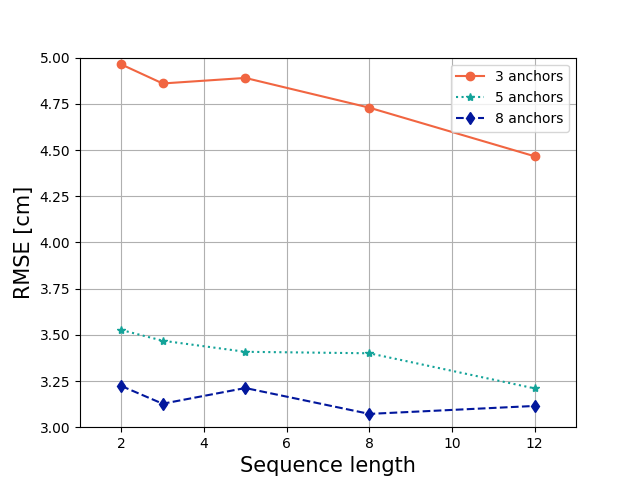
\includegraphics[width=0.9\linewidth]{image/RMSE_error}
	\caption{Plot of Root-Mean-Square-Error (RMSE) with respect to the sequence length for various numbers of anchors.}
	\label{fig:seq_length_on_different_anchors} 	
\end{figure}

We also considered the sequence length as a type of hyperparameters. We investigated the effectiveness of the optimal size of the sequence length by changing the number of input range  data. As Fig. \ref{fig:seq_length_on_different_anchors} shows, the performance is improved when the number of sensors used as input is increased, and as the sequence becomes longer, the network improves the overall performance in accordance with more useful temporal information.

As a result, the networks with longer sequence lengths tend to have smaller error variances and increased abilities to generalize the situation since they can utilize an extended range of temporal information. By doing so, the neural network is able to suppress the disturbance caused by noise. 

\begin{figure*}[h]
	\centering
	\begin{subfigure}[b]{0.32\textwidth}
		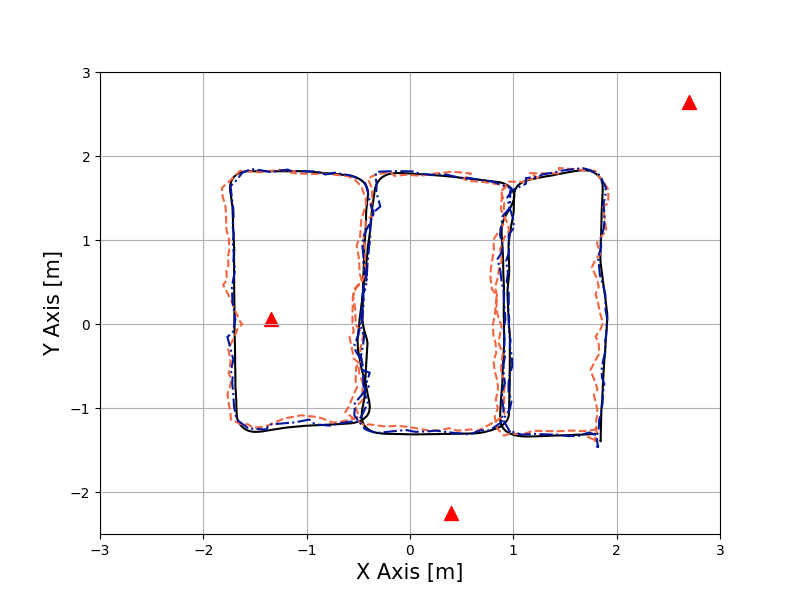
\includegraphics[width=\textwidth]{image/trajectory_3}
		\caption{}
		\label{fig:anchor_3}
	\end{subfigure}
	%add desired spacing between images, e. g. ~, \quad, \qquad, \hfill etc. 
	%(or a blank line to force the subfigure onto a new line)
	\begin{subfigure}[b]{0.32\textwidth}
		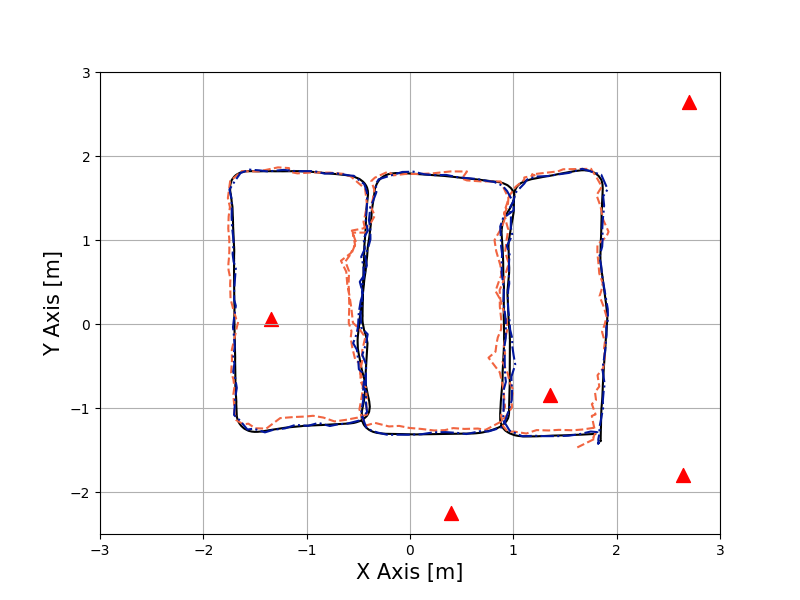
\includegraphics[width=\textwidth]{image/trajectory_5}
		\caption{}
		\label{fig:anchor_5}
	\end{subfigure}
	%add desired spacing between images, e. g. ~, \quad, \qquad, \hfill etc. 
	%(or a blank line to force the subfigure onto a new line)
	\begin{subfigure}[b]{0.32\textwidth}
		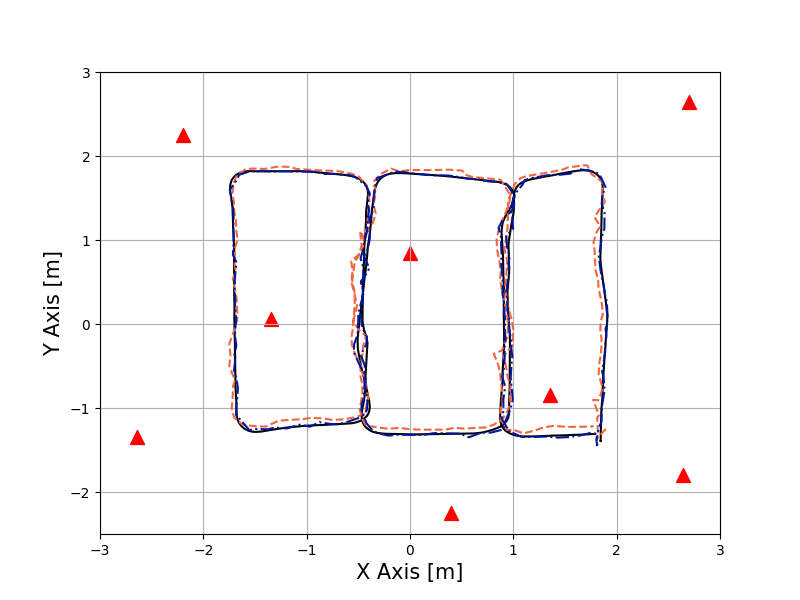
\includegraphics[width=\textwidth]{image/trajectory_8}
		\caption{}
		\label{fig:anchor_8}
	\end{subfigure}
	\caption{Trajectories corresponding to various numbers of anchors: (a) three anchors, (b) five anchors, and (c) eight anchors. For clarity, only the PF-based (orange) and our RONet results (blue) are presented.}\label{fig:trajectories_358}
\end{figure*}

\begin{table*}[h]
	\centering
	\caption{Root-Mean-Square-Error of each algorithm w.r.t. the number of anchors}
	\begin{tabular}{ccccc}
		\toprule
		\multicolumn{5}{c}{RMSE {[}cm{]}}   \\ \midrule
		Number of anchors & Particle Filter\cite{gonzalez2009mobile} & MLP\cite{kumar2016localization} & Bi-LSTM\cite{lim2018effective} & RONet (Ours) \\ \cmidrule{2-5} 
		3             & 8.722 & 5.485 & 5.051 & \textbf{4.466} \\
		5             & 8.286 & 4.546 & 4.418 & \textbf{3.210} \\
		8             & 7.650 & 4.235 & 4.290 & \textbf{3.090} \\ \bottomrule
	\end{tabular}
	\label{table:rmse}
\end{table*}

However, note that the performance of the network becomes inaccurate when the sequence length is set to 12 compared to sequence lengths equal to eight. This might be because of the accumulations of different patterns of sensor noise levels as the number of anchors increases. In other words, the tendency of the domain values may vary owing to the accumulation of different patterns of sensor noise levels, even though a part of the test data path is similar to the path of the train data. This is the reason why range observations included in test data are not correctly or easily mapped following training as sequence length increases.


For these reasons, we set the optimal sequence length to eight. Accordingly, we could somehow address uncertainty issues based on the use of additional temporal information for more precise estimated position.

%Similarily, as sequence length become shorter, it is less difficult for the neural architecture to understand the chracteristics of the sequential data by virtue of the less accumulation of different patterns of system noises. Note that in most cases, the network constructed by the shorter sequential length tend to estimate the position more precisely than those with longer sequential lengths. However, 생t becomes a double-edged sword because temporal information is also reduced accordingly in such a way as to week to the noises, having larger error variance.



%sequence length가 길어질수록 netowrk가 그 sequential data를 일반화 시키는 게 어렵다
%In other workds, sequence length만큼 끊어서 input으로 받기 때문에 sequential한 경향성에 대해 적절한 output을 내게 학습을 하는데, sequence가 길어지게 되면 길어지는 만큼 그 상황이 특수해져서 비슷한 특성을 지닌 input이 줄기 때문이다????
%길이가 길어짐에 따라 noise에 대한 방해를 더 길어진 temporal information을 활용해서 억누를 수 있다.
%On the other hand, 짧아질수록 좋지만 경향성을 학습?


\subsubsection{Performance comparison of other algorithms}

We also compared our network with recently presented learning-based approaches: MLP \cite{kumar2016localization}, Bi--LSTM \cite{lim2018effective}, and the conventional PF-based approach\cite{gonzalez2009mobile, blanco2008pure}. We implemented PF-based localization based on a prior publication of \cite{gonzalez2009mobile}. We tested various numbers of anchors to check the algorithms on the tested environment according to the number of range sensors.

\begin{figure}[h]
	\centering
	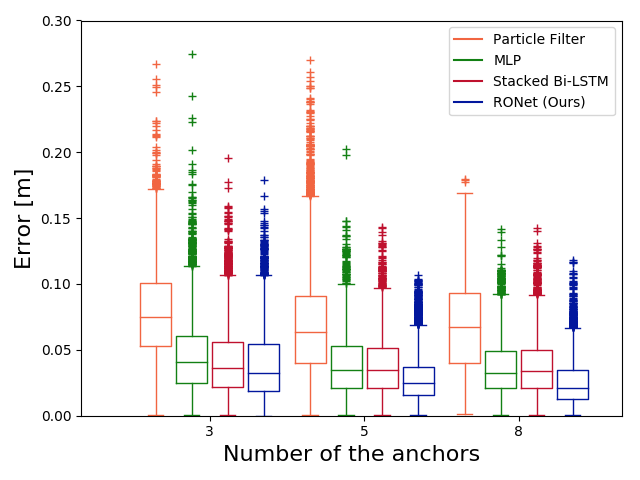
\includegraphics[width=0.9\linewidth]{image/boxcompare}
	\caption{Box plot of results w.r.t. number of anchors.}
	\label{fig:box_plot} 	
\end{figure}

As Fig. \ref{fig:box_plot} and Table \ref{table:rmse} show, our proposed RONet exhibits the best performance among the conventional algorithms and deep learning-based approaches in all cases. RONet yields the smallest RMSE values. Specifically, the RMSE values are 4.466 cm, 3.210 cm, and 3.090 cm, in the cases where three, five, and eight anchors are deployed, respectively. Furthermore, it also shows that our network estimates position with fewer outliers compared to other algorithms. 

\section{Conclusion}

In this study, we proposed a robust three-stacked Bi--LSTM with residual attention, named as RONet to solve the problem of localization using range measurements only. We tested our approach in a realistic manner and showed that it could estimate the position of the mobile robot in real time at an approximate frequency of 32 Hz using range-only measurements. Unlike the conventional probabilistic-based algorithms, the proposed approach did not need any preprocessing module, such as calibration and outlier rejection, because it mapped the range observation and position in an end-to-end manner.

In addition, we also analyzed the sequence length as a type of hyperparameters. We concluded that a specific sequence length can be found to be optimal compared to other lengths. This was attributed to the fact that when a network was built with the optimal sequence length, the ability of the network to deal with uncertainty following the use of additional temporal information was improved, and the position was estimated with increased precision.

Finally, we compared our RONet approach with other conventional probabilistic approaches and previously presented deep-learning-based algorithms. It was shown that RONet yielded the most precise estimates of robot positions. We set three cases, reduced the number of anchors, and confirmed that our RONet was robust, and yielded the smallest RMSE values. 

In future work, this approach should be improved for arbitrary placement of anchor nodes. Besides, this approach should also consider NLOS situation when training RONet. Therefore, the loss term or architecture of the neural network of the proposed method needs to be revised to obtain precise position estimates irrespective of the placement of the anchors or changes in their locations and train data should be acquired considering NLOS cases.

\bibliographystyle{IEEEtran}
% argument is your BibTeX string definitions and bibliography database(s)
\bibliography{./IROS_RObib,./IEEEabrv}


\end{document}
